\documentclass[11pt]{article}

\usepackage[spanish]{babel}
\usepackage[utf8]{inputenc}
\usepackage[T1]{fontenc}
\usepackage{graphicx}
\usepackage{hyperref}
\usepackage{amsmath}
\usepackage{natbib}
\usepackage{caption}
\usepackage{subcaption}
\usepackage[margin=2.5cm]{geometry}

\title{Explicabilidad de un clasificador de imágenes mediante SHAP\\
\large Un estudio de caso con ConvNeXt-Tiny sobre fotografías de gatos}
\author{
  [Mónica Salvatierra] \\{} Responsible AI, [22249] \\{}
  \and
  [Bianca Calderón] \\{} Responsible AI, [22272] \\{}
}
\date{\today}

\begin{document}

\maketitle

\begin{abstract}
Este trabajo presenta un análisis de explicabilidad aplicado a un clasificador de imágenes preentrenado, utilizando el método SHAP (SHapley Additive exPlanations) para identificar qué regiones de una imagen influyen en la predicción del modelo. Se emplea la arquitectura ConvNeXt-Tiny, obtenida del repositorio de Hugging Face, sobre tres fotografías de gatos con distintos patrones de pelaje y distintos fondos. El objetivo central es determinar si el modelo basa sus predicciones en rasgos anatómicos del animal o si, por el contrario, se apoya en atajos visuales como el color del pelaje o elementos del entorno, un fenómeno conocido en la literatura como \emph{shortcut learning}. Los resultados se discuten en el contexto de la inteligencia artificial responsable, dado que la identificación de estos atajos es relevante para evaluar la confiabilidad de un modelo antes de su despliegue.
\end{abstract}

\section{Introducción}

Los modelos de aprendizaje profundo alcanzan niveles de precisión elevados en tareas de clasificación de imágenes, aunque su naturaleza de caja negra dificulta comprender el razonamiento detrás de cada predicción. Esta opacidad representa un riesgo cuando dichos modelos se despliegan en contextos donde una decisión errónea tiene consecuencias reales, por lo que la explicabilidad se ha convertido en un componente central de la inteligencia artificial responsable.

Un problema documentado en la literatura es el \emph{shortcut learning} \citep{geirhos2020shortcut}, que ocurre cuando un modelo aprende una correlación espuria presente en los datos de entrenamiento en lugar del concepto que se pretende que aprenda. El ejemplo más citado en este ámbito es el de un clasificador que distingue lobos de huskies basándose en la presencia de nieve en el fondo de la imagen en vez de las características del animal \citep{ribeiro2016why}. Este trabajo busca explorar si un fenómeno similar ocurre en un clasificador de imágenes preentrenado al enfrentarlo a fotografías de gatos con pelajes y fondos heterogéneos.

Para ello se utiliza SHAP \citep{lundberg2017unified}, un método de explicabilidad basado en la teoría de juegos que asigna a cada región de la imagen una contribución a la predicción final del modelo. La pregunta que guía este análisis es la siguiente. ¿El modelo se basa en rasgos anatómicos del gato, como la forma de la cara, las orejas o los ojos, para realizar su clasificación, o se apoya en atajos visuales como el color del pelaje o elementos del fondo?

\section{Metodología}

\subsection{Modelo}

Se utilizó ConvNeXt-Tiny \citep{liu2022convnet}, una arquitectura convolucional moderna disponible en el repositorio de Hugging Face bajo el identificador \texttt{facebook/convnext-tiny-224}. El modelo fue preentrenado sobre ImageNet \citep{deng2009imagenet} y no recibió ningún ajuste adicional para este trabajo. Se optó por esta arquitectura porque conserva la estructura convolucional clásica, lo cual favorece la generación de mapas de atribución espacialmente coherentes, y porque su tamaño reducido permite ejecutar el análisis SHAP en un tiempo razonable sobre hardware sin aceleración por GPU. El modelo se cargó mediante la librería \texttt{transformers} \citep{wolf2020transformers}.

\subsection{Casos de estudio}

Se seleccionaron tres fotografías, cada una correspondiente a un gato distinto, con el propósito de cubrir patrones de pelaje diferenciados.

\begin{itemize}
  \item \textbf{Gato A.} Pelaje bicolor blanco y negro, de tipo \emph{tuxedo}, fotografiado sobre césped.
  \item \textbf{Gato B.} Pelaje atigrado combinado con blanco, fotografiado en un ambiente interior sobre una alfombra.
  \item \textbf{Gato C.} Pelaje atigrado sólido sin manchas blancas, fotografiado sobre un muro y con un pañuelo decorativo alrededor del cuello.
\end{itemize}

La inclusión del pañuelo en la fotografía del Gato C fue deliberada, ya que introduce un elemento ajeno a la anatomía del animal que permite evaluar si el modelo le asigna relevancia indebida durante la clasificación.

\subsection{Explicabilidad mediante SHAP}

Para cada imagen se calcularon los valores SHAP correspondientes a las clases con mayor probabilidad predicha por el modelo. El procedimiento enmascara progresivamente distintas regiones de la imagen y observa el efecto de dicho enmascaramiento sobre la salida del modelo, lo que permite atribuir a cada región una contribución positiva o negativa hacia la predicción. El resultado se visualiza como un mapa de calor superpuesto a la imagen original, en el que las regiones en tonos cálidos incrementan la probabilidad de la clase evaluada y las regiones en tonos fríos la reducen.

\section{Resultados}

Para cada imagen se reportan las cinco clases con mayor probabilidad predicha por el modelo, seguidas de la descripción del mapa de atribución SHAP correspondiente a las tres clases más probables.

\subsection{Gato A}

El modelo asignó la mayor probabilidad a la clase Egyptian cat, con un valor de 0.4975, seguida de Border collie con 0.1233, doormat welcome mat con 0.0503, collie con 0.0435 y tabby tabby cat con 0.0195. Resulta notable que dos de las cinco clases con mayor probabilidad correspondan a razas de perro, lo cual sugiere que el modelo no identificó con claridad la especie del animal.

El mapa SHAP de la figura \ref{fig:gato-a} muestra que la clase Egyptian cat recibe una contribución positiva concentrada en la región de la cabeza del animal, particularmente alrededor del hocico y los ojos, lo que indica que el modelo se apoya en rasgos faciales para esta predicción. En contraste, la clase Border collie recibe una contribución negativa sobre el pecho blanco del gato y una contribución positiva dispersa hacia los bordes de la imagen, de manera que la coloración bicolor del pelaje parece influir en la probabilidad asignada a esta raza canina, dado que Border collie es una raza reconocida por presentar un patrón de pelaje blanco y negro similar al del animal fotografiado. La clase doormat welcome mat, por su parte, recibe una contribución débil y dispersa a lo largo de toda la imagen, sin concentrarse en una región identificable.

\begin{figure}[h!]
  \centering
  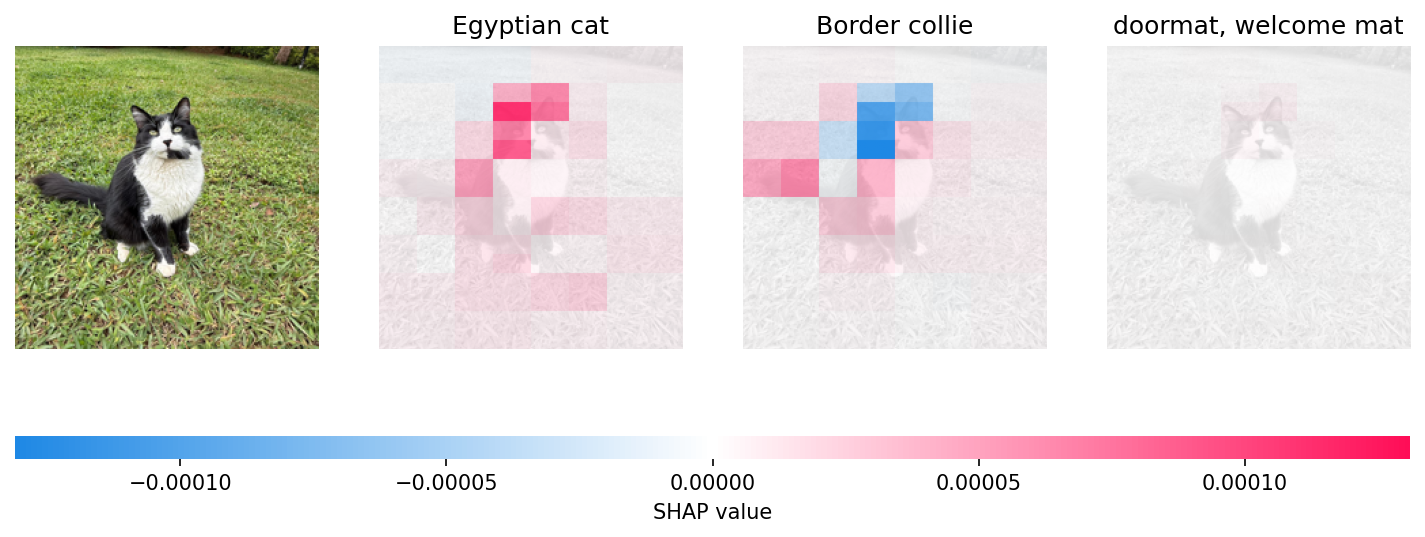
\includegraphics[width=0.8\textwidth]{figures/shap_gato_a_tuxedo.png}
  \caption{Mapa de atribución SHAP para el Gato A.}
  \label{fig:gato-a}
\end{figure}

\subsection{Gato B}

El modelo asignó la mayor probabilidad a la clase tabby tabby cat, con un valor de 0.3760, seguida de Egyptian cat con 0.1768, doormat welcome mat con 0.1590, tiger cat con 0.0959 y lynx catamount con 0.0085. En este caso las cinco clases con mayor probabilidad corresponden a felinos o a un objeto del entorno doméstico, sin que aparezcan razas caninas entre ellas.

Según la figura \ref{fig:gato-b}, la clase tabby tabby cat recibe una contribución positiva concentrada en el dorso del animal, donde el patrón de rayas es más visible, mientras que el pecho blanco recibe una contribución negativa. Esto sugiere que, a diferencia del caso anterior, el modelo asocia correctamente esta clase con el patrón de pelaje atigrado en lugar de con las zonas blancas. La clase Egyptian cat presenta un patrón de atribución similar, aunque con una magnitud menor. La clase doormat welcome mat recibe una contribución mixta y dispersa sobre el cuerpo del animal, sin concentrarse claramente en la alfombra del fondo, por lo que no puede afirmarse con certeza que el fondo textil sea la causa directa de esta predicción, aunque su presencia entre las clases más probables constituye evidencia indirecta de que el entorno de la fotografía influye en la salida del modelo.

\begin{figure}[h!]
  \centering
  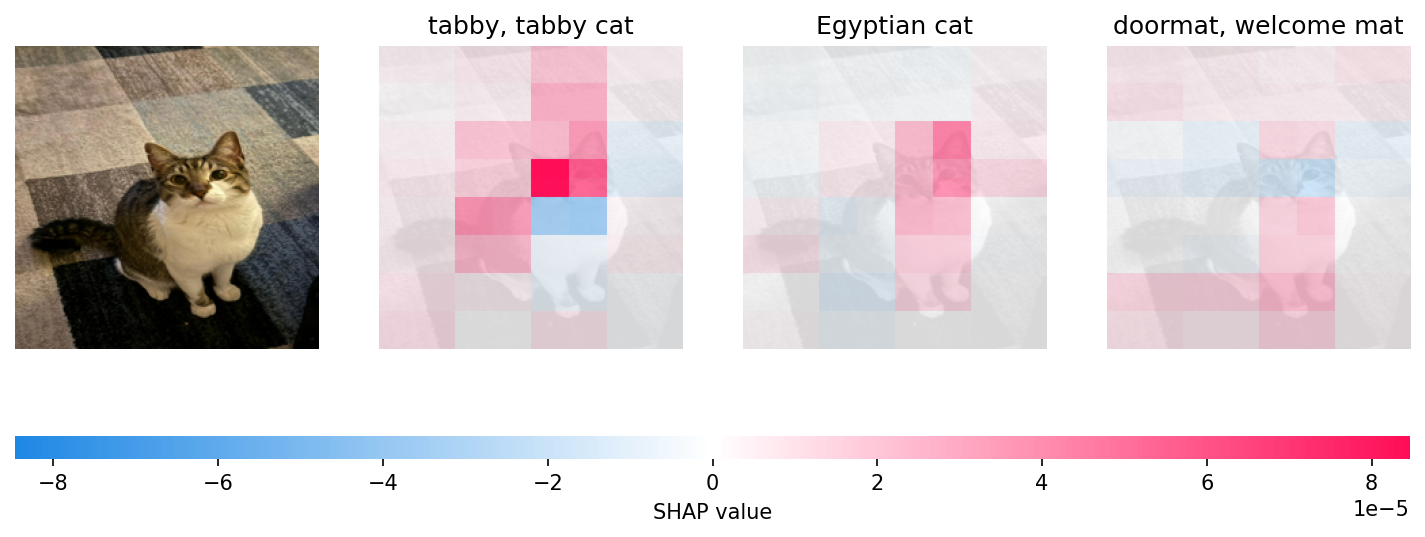
\includegraphics[width=0.8\textwidth]{figures/shap_gato_b_atigrado_blanco.png}
  \caption{Mapa de atribución SHAP para el Gato B.}
  \label{fig:gato-b}
\end{figure}

\subsection{Gato C}

El modelo asignó la mayor probabilidad a la clase tabby tabby cat, con un valor de 0.5396, seguida de tiger cat con 0.1977, Egyptian cat con 0.1306, lynx catamount con 0.0049 y chainlink fence con 0.0024. A diferencia de los dos casos anteriores, las tres clases más probables corresponden por completo a razas o variedades de gato, y la única clase ajena al animal, chainlink fence, recibe una probabilidad marginal.

La figura \ref{fig:gato-c} muestra que las tres clases explicadas concentran su contribución en la región del cuello y la cabeza del animal, precisamente donde se ubica el pañuelo decorativo. La clase tabby tabby cat presenta la contribución positiva más intensa en esa zona. Dado que el pañuelo constituye un elemento ajeno a la anatomía del gato, esta concentración de atribución alrededor del cuello indica que el modelo no ignora por completo los elementos añadidos a la imagen, aunque en este caso dicha influencia no fue suficiente para desplazar la predicción hacia una clase no felina.

\begin{figure}[h!]
  \centering
  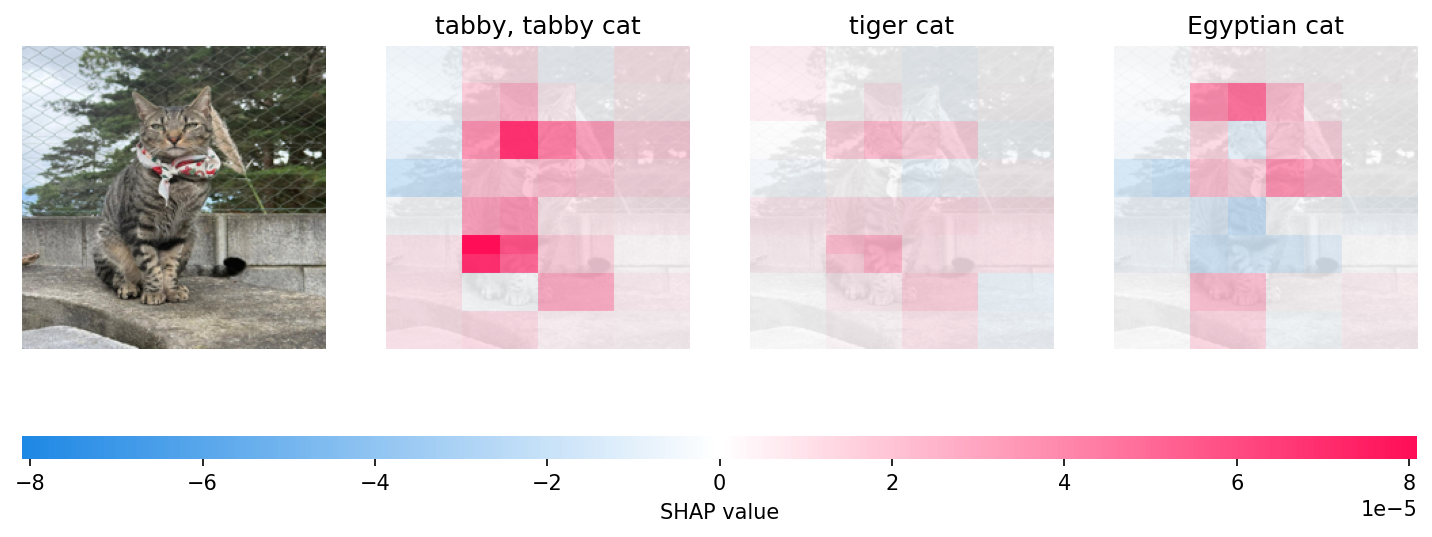
\includegraphics[width=0.8\textwidth]{figures/shap_gato_c_atigrado_solido.png}
  \caption{Mapa de atribución SHAP para el Gato C.}
  \label{fig:gato-c}
\end{figure}

\section{Discusión}

Los tres casos analizados permiten responder de manera parcial la pregunta planteada en la introducción sobre si el modelo se basa en rasgos anatómicos del gato o en atajos visuales como el color del pelaje o el fondo de la imagen.

El caso del Gato A constituye la evidencia más clara de un atajo visual, ya que el modelo asignó una probabilidad considerable a dos razas de perro cuyo rasgo distintivo es precisamente un pelaje bicolor blanco y negro. El mapa SHAP respalda esta interpretación, dado que la contribución hacia la clase Border collie se concentra en la zona de transición entre el pelaje negro y el pecho blanco, en lugar de concentrarse en rasgos faciales o corporales propios de un felino. Por lo tanto, en este caso el color del pelaje parece pesar más que la anatomía del animal.

Los casos del Gato B y del Gato C, en cambio, muestran un comportamiento más cercano al esperado de un clasificador que atiende a rasgos anatómicos, ya que las clases con mayor probabilidad corresponden en su mayoría a variedades de gato y los mapas SHAP se concentran sobre el cuerpo del animal. Sin embargo, la aparición reiterada de la clase doormat welcome mat, presente entre las cinco clases más probables tanto para el Gato A como para el Gato B, sugiere que el modelo conserva cierta sensibilidad a las texturas del fondo, en particular a superficies con patrones repetitivos como el césped o la alfombra. Esta observación no permite concluir que el fondo determine la predicción final, pero sí constituye evidencia de que el contexto de la imagen no es completamente irrelevante para el modelo.

En conjunto, los resultados indican que el comportamiento del modelo no es uniforme entre los tres casos. Mientras que en el Gato C la predicción parece depender principalmente de rasgos asociados al pelaje atigrado y no se ve alterada por un elemento distractor como el pañuelo, en el Gato A el color del pelaje sí condujo a una confusión de especie. Esto sugiere que la presencia de atajos visuales en este modelo depende en buena medida de qué tan atípico resulta el patrón de pelaje del animal fotografiado respecto a las categorías felinas disponibles en ImageNet.

\section{Limitaciones}

El análisis presentado tiene alcances acotados que conviene precisar. En primer lugar, el tamaño de la muestra se limita a tres fotografías, por lo que las conclusiones no pueden generalizarse a la totalidad del comportamiento del modelo frente a imágenes de gatos. En segundo lugar, ImageNet no incluye una categoría genérica para la clase gato, sino razas específicas, de modo que una predicción alejada de la raza real del animal no constituye necesariamente evidencia de un atajo visual, ya que también puede reflejar una limitación propia del conjunto de categorías disponibles. En tercer lugar, el método SHAP utilizado aproxima los valores de Shapley mediante muestreo, dado que un cálculo exacto resulta computacionalmente inviable para modelos de esta complejidad, por lo que los mapas de atribución obtenidos están sujetos a cierta variabilidad entre ejecuciones. Finalmente, el análisis se restringe a una sola arquitectura de modelo, de manera que no es posible determinar si los patrones observados son propios de ConvNeXt-Tiny o se extienden a otras familias de clasificadores.

\section{Conclusión}

Este trabajo utilizó SHAP para examinar si un clasificador de imágenes basado en ConvNeXt-Tiny se apoya en rasgos anatómicos del gato o en atajos visuales al clasificar fotografías de tres animales con patrones de pelaje distintos. Los resultados muestran que el comportamiento del modelo no es homogéneo. En el caso del gato con pelaje bicolor blanco y negro, el modelo asignó una probabilidad considerable a razas caninas con un patrón de color similar, y el mapa de atribución respalda que dicha confusión se origina en el color del pelaje y no en la forma del animal. En los otros dos casos, en contraste, las predicciones y los mapas de atribución se concentraron consistentemente sobre variedades de gato, incluso ante la presencia de un elemento distractor como un pañuelo decorativo.

Esta heterogeneidad es relevante para la inteligencia artificial responsable, ya que ilustra que un mismo modelo puede basar sus decisiones en rasgos anatómicos genuinos en unos casos y en atajos visuales espurios en otros, sin que ambos comportamientos sean evidentes a partir de la precisión reportada por el modelo. La adopción de herramientas de explicabilidad como SHAP permite identificar estos casos particulares antes de que un modelo se despliegue en un contexto donde una decisión basada en un atajo visual tenga consecuencias prácticas.

\section*{Log de prompts y proceso de desarrollo}

El registro completo de las decisiones tomadas durante la construcción de este trabajo, incluyendo la selección del modelo, la selección de las imágenes y los ajustes metodológicos discutidos durante el proceso, se documenta en el archivo \texttt{prompt\_log.md} incluido en el paquete entregable.

\bibliographystyle{plainnat}
\bibliography{references}

\end{document}
